% This file was created by tikzplotlib v0.9.8.
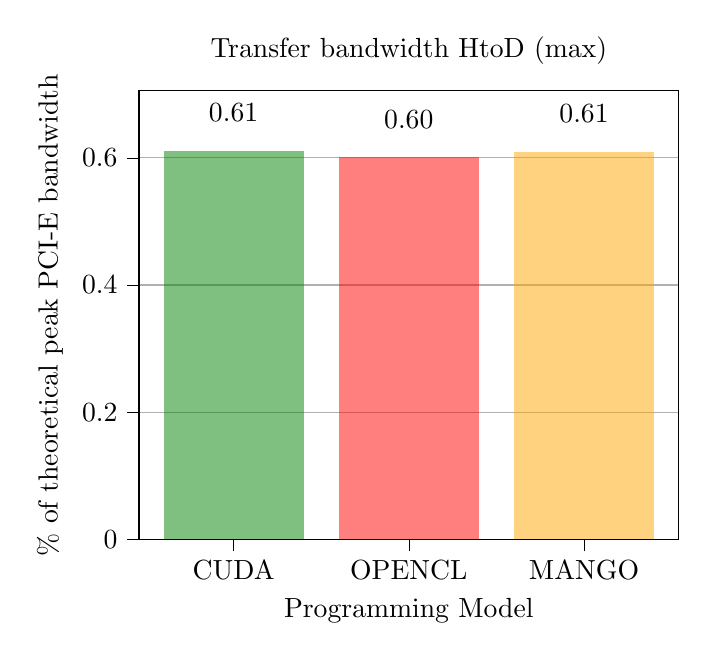
\begin{tikzpicture}

\definecolor{color0}{rgb}{1,0.647058823529412,0}

\begin{axis}[
tick align=outside,
tick pos=left,
title={Transfer bandwidth HtoD (max)},
x grid style={white!69.0196078431373!black},
xlabel={Programming Model},
xmin=-0.54, xmax=2.54,
xtick style={color=black},
xtick={0,1,2},
xticklabels={CUDA,OPENCL,MANGO},
y grid style={white!69.0196078431373!black},
ylabel={\% of theoretical peak PCI-E bandwidth},
ymajorgrids,
ymin=0, ymax=0.70542003271812,
ytick style={color=black}
]
\draw[draw=none,fill=green!50.1960784313725!black,fill opacity=0.5] (axis cs:-0.4,0) rectangle (axis cs:0.4,0.610923870235901);
\draw[draw=none,fill=red,fill opacity=0.5] (axis cs:0.6,0) rectangle (axis cs:1.4,0.60100675941772);
\draw[draw=none,fill=color0,fill opacity=0.5] (axis cs:1.6,0) rectangle (axis cs:2.4,0.610093486271566);
\draw (axis cs:0,0.641290938834655) node[
  scale=1,
  anchor=south,
  text=black,
  rotate=0.0
]{0.61};
\draw (axis cs:1,0.631373828016473) node[
  scale=1,
  anchor=south,
  text=black,
  rotate=0.0
]{0.60};
\draw (axis cs:2,0.640460554870319) node[
  scale=1,
  anchor=south,
  text=black,
  rotate=0.0
]{0.61};
\end{axis}

\end{tikzpicture}
